\chapter{1D: domain definition and characterization}



\section{Input domain definition}


\subsection{3D}

\subsubsection{Maps}

\begin{center}
\begin{longtable}{|p {3.5 cm}|p {6.5 cm}|p {3 cm}|p {4 cm}|}
\hline
\textbf{Keyword} & \textbf{Description}  \\ \hline
\endfirsthead
\hline
\multicolumn{4}{| c |}{continued from previous page} \\
\hline
\textbf{Keyword} & \textbf{Description}  \\ \hline
\endhead
\hline
\multicolumn{4}{| c |}{{continued on next page}}\\ 
\hline
\endfoot
\endlastfoot
\hline
DemFile & name of the file providing the DEM map  \\ \hline
LandCoverMapFile & name of the file providing the land cover map  \\ \hline
\caption{Keywords of input file related to the domain}
\label{input_file}
\end{longtable}
\end{center}


\subsubsection{Parameters}

\begin{center}
\begin{longtable}{|p {3.5 cm}|p {4.7 cm}|p {1. cm}|p{0.8 cm}|p{1.4 cm}|p{0.8 cm}|p{1.3 cm}|}
\hline
\textbf{Keyword} & \textbf{Description} & \textbf{M. U.} & \textbf{range} & \textbf{Default Value} & \textbf{Sca / Vec} & \textbf{Str / Num / Opt} \\ \hline
\endfirsthead
\hline
\multicolumn{7}{| c |}{continued from previous page} \\
\hline
\textbf{Keyword} & \textbf{Description} & \textbf{M. U.} & \textbf{range} & \textbf{Default Value} & \textbf{Sca / Vec} & \textbf{Str / Num / Opt} \\ \hline
\endhead
\hline
\multicolumn{7}{| c |}{{continued on next page}}\\ 
\hline
\endfoot
\endlastfoot
\hline
%PointSoilType & Soil type of the simulation point & - &  & NA & vec & num \\ \hline
SoilLayerThicknesses \index{SoilLayerThicknesses} & vector defining the thickness of the various soil layers. If not present, a column of 5 layers 100 mm thick will be assumed & mm &  & 100 & vec & num \\ \hline
SoilLayerNumber \index{SoilLayerNumber} & number of soil layers (is calculated after the number of components of the vector SoilLayerNumber) & - &  & 5 & sca & num \\ \hline
\caption{Keywords of  parameters referred to soil layer}
\label{domain_parameters1D_numeric}
\end{longtable}
\end{center}

\subsection{1D}

\subsubsection{Parameters}

\begin{center}
\begin{longtable}{|p {3.5 cm}|p {4.7 cm}|p {1. cm}|p{0.8 cm}|p{1.4 cm}|p{0.8 cm}|p{1.3 cm}|}
\hline
\textbf{Keyword} & \textbf{Description} & \textbf{M. U.} & \textbf{range} & \textbf{Default Value} & \textbf{Sca / Vec} & \textbf{Str / Num / Opt} \\ \hline
\endfirsthead
\hline
\multicolumn{7}{| c |}{continued from previous page} \\
\hline
\textbf{Keyword} & \textbf{Description} & \textbf{M. U.} & \textbf{range} & \textbf{Default Value} & \textbf{Sca / Vec} & \textbf{Str / Num / Opt} \\ \hline
\endhead
\hline
\multicolumn{7}{| c |}{{continued on next page}}\\ 
\hline
\endfoot
\endlastfoot
\hline
%PointSoilType & Soil type of the simulation point & - &  & NA & vec & num \\ \hline
SoilLayerThicknesses & vector defining the thickness of the various soil layers. If not present, a column of 5 layers 100 mm thick will be assumed & mm &  & 100 & vec & num \\ \hline
SoilLayerNumber & number of soil layers (is calculated after the number of components of the vector SoilLayerNumber) & - &  & 5 & sca & num \\ \hline
\caption{Keywords of parameters referred to soil layer}
\label{domain_parameters3D_numeric}
\end{longtable}
\end{center}


\section{Input}

\subsection{1D without maps}


\subsubsection{Parameters}
\begin{center}
\begin{longtable}{|p {5.5 cm}|p {3. cm}|p {1.2 cm}|p{1.0 cm}|p{1.2 cm}|p{0.8 cm}|p{1. cm}|}
\hline
\textbf{Keyword} & \textbf{Description} & \textbf{M. U.} & \textbf{range} & \textbf{Default Value} & \textbf{Sca / Vec} & \textbf{Log / Num} \\ \hline
\endfirsthead
\hline
\multicolumn{7}{| c |}{continued from previous page} \\
\hline
\textbf{Keyword} & \textbf{Description} & \textbf{M. U.} & \textbf{range} & \textbf{Default Value} & \textbf{Sca / Vec} & \textbf{Log / Num} \\ \hline
\endhead
\hline
\multicolumn{7}{| c |}{{continued on next page}}\\ 
\hline
\endfoot
\endlastfoot
\hline
PointLandCoverType \index{PointLandCoverType} & Land Cover type of the simulation point & - &  & NA & vec & num \\ \hline
PointSoilType \index{PointSoilType} & Soil type of the simulation point & - &  & NA & vec & num \\ \hline
PointElevation \index{PointElevation} & elevation of the point of simulation & m a.s.l. &  & NA & vec & num \\ \hline
PointSlope \index{PointSlope} & Slope steepness of the simulation point & degree &  & NA & vec & num \\ \hline
PointAspect \index{PointAspect} & Aspect of the simulation point & degree &  & NA & vec & num \\ \hline
PointSkyViewFactor \index{PointSkyViewFactor}& Sky View Factor of the simulation point & - &  & NA & vec & num \\ \hline
PointCurvatureNorthSouthDirection \index{PointCurvatureNorthSouthDirection} & N-S curvature of the simulation point & m$^{-1}$ &  & NA & vec & num \\ \hline
PointCurvatureWestEastDirection \index{PointCurvatureWestEastDirection} & W-E curvature of the simulation point & m$^{-1}$ &  & NA & vec & num \\ \hline
PointCurvatureNorthwestSoutheastDirection \index{PointCurvatureNorthwestSoutheastDirection}& N-W curvature of the simulation point & m$^{-1}$ &  & NA & vec & num \\ \hline
PointCurvatureNortheastSouthwestDirection \index{PointCurvatureNortheastSouthwestDirection} & N-E curvature of the simulation point & m$^{-1}$ &  & NA & vec & num \\ \hline
PointDrainageLateralDistance \index{PointDrainageLateralDistance} & Lateral Drainage distance of the simulation point & m &  & NA & vec & num \\ \hline
PointLatitude \index{PointLatitude} & Latitude of the simulation point & degree &  & NA & vec & num \\ \hline
PointLongitude \index{PointLongitude} & Longitude of the simulation point & degree &  & NA & vec & num \\ \hline
PointHorizon \index{PointHorizon} & number of the HorizonPointFile that describes the horizon of the simulation point & - &  & NA & vec & num \\ \hline
\caption {Keywords of topographical, land cover and soil type characteristics that may be set in geotop.inpts. Each parameter may be give in input as a vector, each component representing a point. Otherwise the characteristics may be summarized in the file PointFile, each value corresponding to the proper header defined in Table \ref{headers_topo_par1D}. }
\label{topo_par1d_topo}
\end{longtable}
\end{center}


\begin{center}
\begin{longtable}{|p {3.3 cm}|p {4.7 cm}|p {1.7 cm}|p{1.0 cm}|p{1.2 cm}|p{0.8 cm}|p{1. cm}|}
\hline
\textbf{Keyword} & \textbf{Description} & \textbf{M. U.} & \textbf{range} & \textbf{Default Value} & \textbf{Scalar / Vector} & \textbf{Logical / Numeric} \\ \hline
\endfirsthead
\hline
\multicolumn{7}{| c |}{continued from previous page} \\
\hline
\textbf{Keyword} & \textbf{Description} & \textbf{M. U.} & \textbf{range} & \textbf{Default Value} & \textbf{Scalar / Vector} & \textbf{Logical / Numeric} \\ \hline
\endhead
\hline
\multicolumn{7}{| c |}{{continued on next page}}\\ 
\hline
\endfoot
\endlastfoot
\hline
\caption{Table of topographic parameters  (numeric)}
\label{topo1d_topo_par}
\end{longtable}
\end{center}


\subsubsection{Files}

\begin{center}
\begin{longtable}{|p {2.5 cm}|p {8.5 cm}|p {1 cm}|p {1 cm}|}
\hline
\textbf{Keyword} & \textbf{Description}  \\ \hline
\endfirsthead
\hline
\multicolumn{4}{| c |}{continued from previous page} \\
\hline
\textbf{Keyword} & \textbf{Description}  \\ \hline
\endhead
\hline
\multicolumn{4}{| c |}{{continued on next page}}\\ 
\hline
\endfoot
\endlastfoot
\hline
PointFile \index{PointFile} & name of the file providing the properties for the simulation point  \\ \hline
HorizonPointFile \index{HorizonPointFile} & name of the file providing the horizon of the simulation point  \\ \hline
\caption{Keywords of files related to soil/rock spatial characterization for 1D simulation}
\label{key1D_data}
\end{longtable}
\end{center}

\subsubsection{Headers}

\begin{center}
\begin{longtable}{|p {6.5 cm}|p {6 cm}|p {2 cm}|p {1 cm}|}
\hline
\textbf{Keyword} & \textbf{Description} & \textbf{Associated file}  \\ \hline
\endfirsthead
\hline
\multicolumn{4}{| c |}{continued from previous page} \\
\hline
\textbf{Keyword} & \textbf{Description} & \textbf{Associated file}  \\ \hline
\endhead
\hline
\multicolumn{4}{| c |}{{continued on next page}}\\ 
\hline
\endfoot
\endlastfoot
\hline
HeaderHorizonAngle \index{HeaderHorizonAngle} & String representing the header of the column HorizonAngle of the HorizonPoint and HorizonMeteoStation files & HorizonPoint / HorizonMeteoStation  \\ \hline
HeaderHorizonHeight \index{HeaderHorizonHeight} & String representing the header of the column HorizonHeight of the HorizonPoint and HorizonMeteoStation files & HorizonPoint / HorizonMeteoStation  \\ \hline
HeaderPointElevation \index{HeaderPointElevation} & column name in the file PointFile for the elevation of the point & PointFile  \\ \hline
HeaderPointSlope \index{HeaderPointSlope} & column name in the file PointFile for the slope steepness of the point & PointFile  \\ \hline
HeaderPointAspect \index{HeaderPointAspect} & column name in the file PointFile for the aspect of the point & PointFile  \\ \hline
HeaderPointSkyViewFactor \index{HeaderPointSkyViewFactor} & column name in the file PointFile for the sky view factor of the point & PointFile  \\ \hline
HeaderPointCurvatureNorthSouthDirection \index{HeaderPointCurvatureNorthSouthDirection} & column name in the file PointFile for the N-S curvature of the point & PointFile  \\ \hline
HeaderPointCurvatureWestEastDirection \index{HeaderPointCurvatureWestEastDirection} & column name in the file PointFile for the E-W curvature of the point & PointFile  \\ \hline
HeaderPointCurvatureNorthwestSoutheastDirection \index{HeaderPointCurvatureNorthwestSoutheastDirection} & column name in the file PointFile for the NW-SE curvature of the point & PointFile  \\ \hline
HeaderPointCurvatureNortheastSouthwestDirection \index{HeaderPointCurvatureNortheastSouthwestDirection} & column name in the file PointFile for the NE-SW curvature of the point & PointFile  \\ \hline
HeaderPointDrainageLateralDistance \index{HeaderPointDrainageLateralDistance} & column name in the file PointFile for the distance of lateral drainage & PointFile  \\ \hline
HeaderPointHorizon \index{HeaderPointHorizon} & column name in the file PointFile that provides the number of the HorizonPointFile that describes the horizon of the simulation point & PointFile  \\ \hline
HeaderPointLatitude \index{HeaderPointLatitude} & column name in the file PointFile for the latitude of the point & PointFile  \\ \hline
HeaderPointLongitude \index{HeaderPointLongitude} & column name in the file PointFile for the longitude of the point & PointFile  \\ \hline
HeaderPointID \index{HeaderPointID} & column name in the file PointFile for the identification ID of the point & PointFile  \\ \hline
HeaderCoordinatePointX \index{HeaderCoordinatePointX} & column name in the file PointFile for the x coordinate of the point & PointFile  \\ \hline
HeaderCoordinatePointY \index{HeaderCoordinatePointY} & column name in the file PointFile for the y coordinate of the point & PointFile  \\ \hline
\caption{Keywords of headers that specify the soil/rock spatial characterization for 1D simulation}
\label{headers_topo_par1D}
\end{longtable}
\end{center}






\subsection{1D with maps}

\subsubsection{Maps}

\begin{center}
\begin{longtable}{|p {3.5 cm}|p {6.5 cm}|p {3 cm}|p {4 cm}|}
\hline
\textbf{Keyword} & \textbf{Description}  \\ \hline
\endfirsthead
\hline
\multicolumn{4}{| c |}{continued from previous page} \\
\hline
\textbf{Keyword} & \textbf{Description}  \\ \hline
\endhead
\hline
\multicolumn{4}{| c |}{{continued on next page}}\\ 
\hline
\endfoot
\endlastfoot
\hline
DemFile \index{DemFile} & name of the file providing the DEM map  \\ \hline
SkyViewFactorMapFile \index{SkyViewFactorMapFile}& name of the file providing the sky view factor map  \\ \hline
SlopeMapFile \index{SlopeMapFile} & name of the file providing the slope steepness map  \\ \hline
RiverNetwork \index{RiverNetwork} & name of the file providing the river network map  \\ \hline
AspectMapFile \index{AspectMapFile} & name of the file providing the aspect map  \\ \hline
CurvaturesMapFile \index{CurvaturesMapFile} & name of the file providing the curvature map  \\ \hline
%BedrockDepthMapFile & name of the file providing the bedrock depth map  \\ \hline
LandCoverMapFile \index{LandCoverMapFile} & name of the file providing the land cover map  \\ \hline
SoilMapFile \index{SoilMapFile} & name of the file providing the soil map  \\ \hline
\caption{Keywords of input file related to the domain}
\label{Input_top_1D_withoutmaps}
\end{longtable}
\end{center}

\subsubsection{Files}

\begin{center}
\begin{longtable}{|p {2.5 cm}|p {8.5 cm}|p {1 cm}|p {1 cm}|}
\hline
\textbf{Keyword} & \textbf{Description}  \\ \hline
\endfirsthead
\hline
\multicolumn{4}{| c |}{continued from previous page} \\
\hline
\textbf{Keyword} & \textbf{Description}  \\ \hline
\endhead
\hline
\multicolumn{4}{| c |}{{continued on next page}}\\ 
\hline
\endfoot
\endlastfoot
\hline
PointFile \index{PointFile} & name of the file providing the properties for the simulation point  \\ \hline
\caption{Keyword of the file related to the spatial characterization of soil/rock properties. The parameters identified by the row index represent the value corresponding to the SoilMapFile map.}
\label{key3D_data_ii}
\end{longtable}
\end{center}


\subsubsection{Parameters}
\begin{center}
\begin{longtable}{|p {2.2 cm}|p {4.2 cm}|p {2.7 cm}|p{1.0 cm}|p{1.2 cm}|p{0.8 cm}|p{1. cm}|}
\hline
\textbf{Keyword} & \textbf{Description} & \textbf{M. U.} & \textbf{range} & \textbf{Default Value} & \textbf{Sca / Vec} & \textbf{Log / Num} \\ \hline
\endfirsthead
\hline
\multicolumn{7}{| c |}{continued from previous page} \\
\hline
\textbf{Keyword} & \textbf{Description} & \textbf{M. U.} & \textbf{range} & \textbf{Default Value} & \textbf{Sca / Vec} & \textbf{Log / Num} \\ \hline
\endhead
\hline
\multicolumn{7}{| c |}{{continued on next page}}\\ 
\hline
\endfoot
\endlastfoot
\hline
PointID \index{PointID}& identification code for the point of simulation &  &  & NA & vec & num \\ \hline
CoordinatePointX \index{CoordinatePointX}& coordinate X if PixelCoordinates is 1, number of row of the matrix if PixelCoordinates is 0 & m (according to the geographical projection of the maps) &  & NA & vec & num \\ \hline
CoordinatePointY \index{CoordinatePointY} & coordinate Y if PixelCoordinates is 1, number of column of the matrix if PixelCoordinates is 1 & m (according to the geographical projection of the maps) &  & NA & vec & num \\ \hline
Latitude \index{Latitude} & Average latitude of the basin, positive means north, negative means south & degree & -90, 90 & 45 & sca & num \\ \hline
Longitude \index{Longitude} & Average longitude of the basin, eastwards from 0 meridiane & degree & 0, 180 & 0 & sca & num \\ \hline
\caption{Keywords of point characterization for the choice of points where to perform a 1D simulation}
\label{topo_par1d_withmaps}
\end{longtable}
\end{center}

\subsubsection{Headers}

\begin{center}
\begin{longtable}{|p {4.15 cm}|p {8 cm}|p {2 cm}|p {1 cm}|}
\hline
\textbf{Keyword} & \textbf{Description} & \textbf{Associated file}  \\ \hline
\endfirsthead
\hline
\multicolumn{4}{| c |}{continued from previous page} \\
\hline
\textbf{Keyword} & \textbf{Description} & \textbf{Associated file}  \\ \hline
\endhead
\hline
\multicolumn{4}{| c |}{{continued on next page}}\\ 
\hline
\endfoot
\endlastfoot
\hline
HeaderPointID \index{HeaderPointID}& column name in the file PointFile for the identification ID of the point & PointFile  \\ \hline
HeaderCoordinatePointX \index{HeaderCoordinatePointX} & column name in the file PointFile for the x coordinate of the point & PointFile  \\ \hline
HeaderCoordinatePointY \index{HeaderCoordinatePointY}& column name in the file PointFile for the y coordinate of the point & PointFile  \\ \hline
\caption{Keywords of headers that specify the soil/rock spatial characterization for 1D simulation}
\label{headers_topo_par1D}
\end{longtable}
\end{center}



\subsection{3D}

\subsubsection{Maps}

\begin{center}
\begin{longtable}{|p {3.5 cm}|p {7 cm}|p {1 cm}|p {1 cm}|}
\hline
\textbf{Keyword} & \textbf{Description}  \\ \hline
\endfirsthead
\hline
\multicolumn{4}{| c |}{continued from previous page} \\
\hline
\textbf{Keyword} & \textbf{Description}  \\ \hline
\endhead
\hline
\multicolumn{4}{| c |}{{continued on next page}}\\ 
\hline
\endfoot
\endlastfoot
\hline
DemFile \index{DemFile}& name of the file providing the DEM map  \\ \hline
SkyViewFactorMapFile \index{SkyViewFactorMapFile}& name of the file providing the sky view factor map  \\ \hline
SlopeMapFile \index{SlopeMapFile} & name of the file providing the slope steepness map  \\ \hline
RiverNetwork \index{RiverNetwork}& name of the file providing the river network map  \\ \hline
AspectMapFile \index{AspectMapFile} & name of the file providing the aspect map  \\ \hline
CurvaturesMapFile \index{CurvaturesMapFile} & name of the file providing the curvature map  \\ \hline
BedrockDepthMapFile \index{BedrockDepthMapFile}& name of the file providing the bedrock depth map  \\ \hline
LandCoverMapFile \index{LandCoverMapFile} & name of the file providing the land cover map  \\ \hline
SoilMapFile \index{SoilMapFile}& name of the file providing the soil map  \\ \hline
\caption{Keywords of input maps necessary to launch the 3D simulation}
\label{key3D_soilrock}
\end{longtable}
\end{center}

\subsubsection{Files}

\begin{center}
\begin{longtable}{|p {2.5 cm}|p {8.5 cm}|p {1 cm}|p {1 cm}|}
\hline
\textbf{Keyword} & \textbf{Description}  \\ \hline
\endfirsthead
\hline
\multicolumn{4}{| c |}{continued from previous page} \\
\hline
\textbf{Keyword} & \textbf{Description}  \\ \hline
\endhead
\hline
\multicolumn{4}{| c |}{{continued on next page}}\\ 
\hline
\endfoot
\endlastfoot
\hline
PointFile \index{PointFile}& name of the file providing the properties for the simulation point  \\ \hline
\caption{Keyword of the file related to the spatial characterization of soil/rock properties. The parameters identified by the row index represent the value corresponding to the SoilMapFile map.}
\label{key3D_data}
\end{longtable}
\end{center}


\subsubsection{Parameters}
\begin{center}
\begin{longtable}{|p {2.3 cm}|p {6. cm}|p {1.5 cm}|p{1.0 cm}|p{1.2 cm}|p{0.8 cm}|p{1. cm}|}
\hline
\textbf{Keyword} & \textbf{Description} & \textbf{M. U.} & \textbf{range} & \textbf{Default Value} & \textbf{Sca / Vec} & \textbf{Log / Num} \\ \hline
\endfirsthead
\hline
\multicolumn{7}{| c |}{continued from previous page} \\
\hline
\textbf{Keyword} & \textbf{Description} & \textbf{M. U.} & \textbf{range} & \textbf{Default Value} & \textbf{Sca / Vec} & \textbf{Log / Num} \\ \hline
\endhead
\hline
\multicolumn{7}{| c |}{{continued on next page}}\\ 
\hline
\endfoot
\endlastfoot
\hline
Latitude \index{Latitude}& Average latitude of the basin, positive means north, negative means south & degree & -90, 90 & 45 & sca & num \\ \hline
Longitude \index{Longitude} & Average longitude of the basin, eastwards from 0 meridiane & degree & 0, 180 & 0 & sca & num \\ \hline
\caption {Keyword of point characterization for 3D simulations}
\label{topo_par3d_gen}
\end{longtable}
\end{center}


\section{Output}


\subsection{3D}
\subsubsection{Headers}

\begin{center}
\begin{longtable}{|p {3.5 cm}|p {4.5 cm}|p {2.5 cm}|p {4 cm}|}
\hline
\textbf{Keyword} & \textbf{Description} & \textbf{Associated file}  \\ \hline
\endfirsthead
\hline
\multicolumn{4}{| c |}{continued from previous page} \\
\hline
\textbf{Keyword} & \textbf{Description} & \textbf{Associated file}  \\ \hline
\endhead
\hline
\multicolumn{4}{| c |}{{continued on next page}}\\ 
\hline
\endfoot
\endlastfoot
\hline
HeaderPointID \index{HeaderPointID}& column name in the file PointFile for the identification ID of the point & PointFile  \\ \hline
HeaderCoordinatePointX \index{HeaderCoordinatePointX} & column name in the file PointFile for the x coordinate of the point & PointFile  \\ \hline
HeaderCoordinatePointY \index{HeaderCoordinatePointY} & column name in the file PointFile for the y coordinate of the point & PointFile  \\ \hline
\caption{Keywords of header that specify the soil/rock spatial characterization for 3D simulation }
\label{header_soilrock3D}
\end{longtable}
\end{center}



\subsubsection{Parameters}
\begin{center}
\begin{longtable}{|p {2.2 cm}|p {4.2 cm}|p {2.7 cm}|p{1.0 cm}|p{1.2 cm}|p{0.8 cm}|p{1. cm}|}
\hline
\textbf{Keyword} & \textbf{Description} & \textbf{M. U.} & \textbf{range} & \textbf{Default Value} & \textbf{Sca / Vec} & \textbf{Log / Num} \\ \hline
\endfirsthead
\hline
\multicolumn{7}{| c |}{continued from previous page} \\
\hline
\textbf{Keyword} & \textbf{Description} & \textbf{M. U.} & \textbf{range} & \textbf{Default Value} & \textbf{Sca / Vec} & \textbf{Log / Num} \\ \hline
\endhead
\hline
\multicolumn{7}{| c |}{{continued on next page}}\\ 
\hline
\endfoot
\endlastfoot
\hline
PointID \index{PointID}& identification code for the point of simulation &  &  & NA & vec & num \\ \hline
CoordinatePointX \index{CoordinatePointX} & coordinate X if PixelCoordinates is 1, number of row of the matrix if PixelCoordinates is 0 & m (according to the geographical projection of the maps) &  & NA & vec & num \\ \hline
CoordinatePointY \index{CoordinatePointY}& coordinate Y if PixelCoordinates is 1, number of column of the matrix if PixelCoordinates is 1 & m (according to the geographical projection of the maps) &  & NA & vec & num \\ \hline
\caption{Keywords of point characterization for the choice of point outputs in 3D simulations}
\label{topo_par3d_gen}
\end{longtable}
\end{center}




%\begin{figure}[h!]
%\begin{center}
%  \begin{minipage}[c]{.65\textwidth}
%    \centering
%    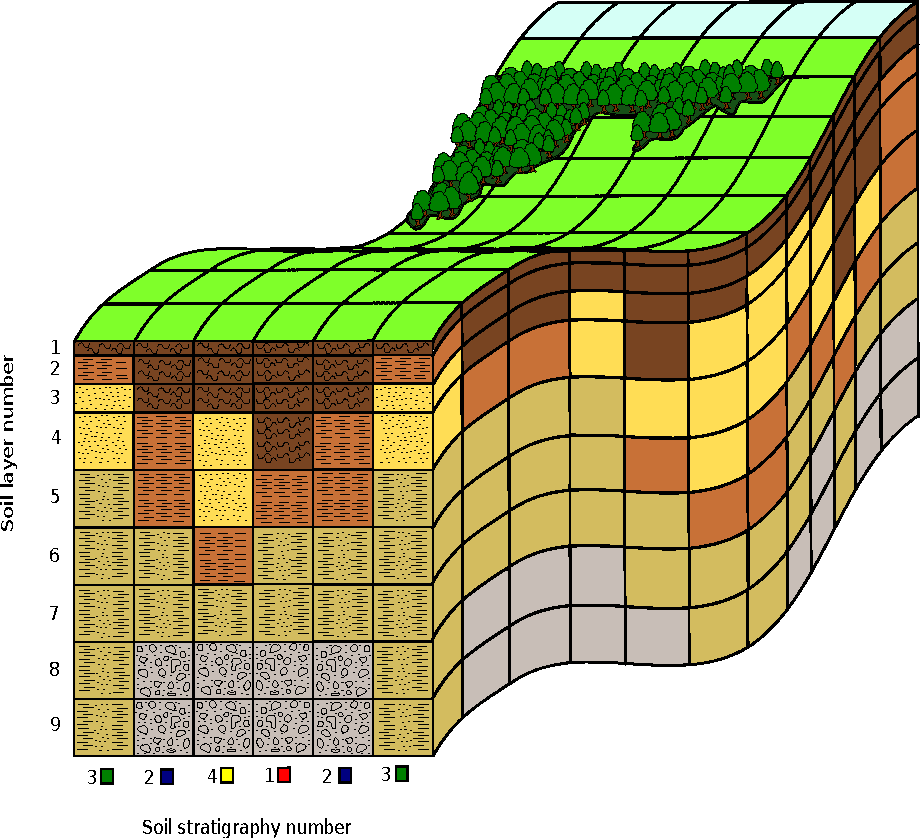
\includegraphics[width=1\textwidth]{./images/pic_spatchar/discretizzazione_3d.pdf}
%  \end{minipage}%
%  \hspace{10mm}%
%  \begin{minipage}[c]{.25\textwidth}
%    \centering
%    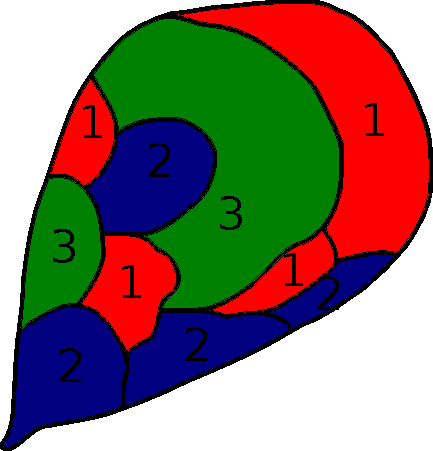
\includegraphics[width=1\textwidth]{./images/pic_spatchar/soil_stratigraphy_basin.pdf}
%  \end{minipage}
%\end{center}
%\textsl{\caption{Soil stratigraphy}\label{ww}}
%\end{figure}


